\documentclass{beamer}

\usepackage[utf8]{inputenc}
\usepackage[T2A]{fontenc}
\usepackage[utf8]{inputenc}
\usepackage[russian]{babel}

\let\vec\mathbf
% \usetheme{Berlin}

\addtobeamertemplate{navigation symbols}{}{%
    \usebeamerfont{footline}%
    \usebeamercolor[fg]{footline}%
    \hspace{1em}%
    \insertframenumber/\inserttotalframenumber
}

\title{Защищенное распределенное умножение матриц с использованием полиномиального кодирования}
\author{Авдотьин Е., Глинский К., Ендовицкий Е.}
\institute{МФТИ}
\date{2019}

\begin{document}
    
    \frame{\titlepage}

    \begin{frame}
        \frametitle{Постановка задачи}
        \begin{itemize}
            \item<1-> \textbf{Клиент}
            \begin{itemize}
                \item Имеет две матрицы: $A \in \mathbb{F}_q^{r\times s}$, $B \in \mathbb{F}_q^{s\times t}$
                \item Хочет получить матрицу $C = AB \in \mathbb{F}_q^{r \times t}$
            \end{itemize}
            \item<2-> \textbf{Серверы}
            \begin{itemize}
                \item Каждый может получать на вход две матрицы и вычислять их произведение
            \end{itemize}
            \item<3-> \textbf{Цель}
            \begin{itemize}
                \item Вычислить $C = AB$ с использованием серверов, при этом ни один из них не должен иметь информацию об $A$ и $B$
                % \item 
            \end{itemize}
        \end{itemize}
    \end{frame}

    \begin{frame}
        \frametitle{Полиномиальное кодирование: пример}
        \begin{itemize}
            \item Имеется две матрицы $A \in \mathbb{F}_q^{r\times s}$, $B \in \mathbb{F}_q^{s\times t}$
            \begin{itemize}
                \item<1-> Сгенерируем две случайные матрицы $R \in \mathbb{F}_q^{r\times s}$, $S \in \mathbb{F}_q^{s\times t}$
                \item<2-> Рассмотрим многочлены
                \begin{equation*}
                    f(x) = A + Rx, \; g(x) = B + Sx
                \end{equation*}
                \item<3-> Их произведение имеет вид
                \begin{equation*}
                    h(x) = f(x) \cdot g(x) = AB + \left(AS + RB\right) + RSx^2
                \end{equation*}
                \item<4-> Имея 3 значения $h$, можно восстановить многочлен $h(x)$ и найти $h(0) = AB$
            \end{itemize}
        \end{itemize}
    \end{frame}

    \begin{frame}

        \frametitle{Распределенное полиномиальное кодирование}
        \begin{itemize}
            \item Вычисление значений $h(x)$ может производиться на распределенных серверах
            \begin{figure}[t!]
                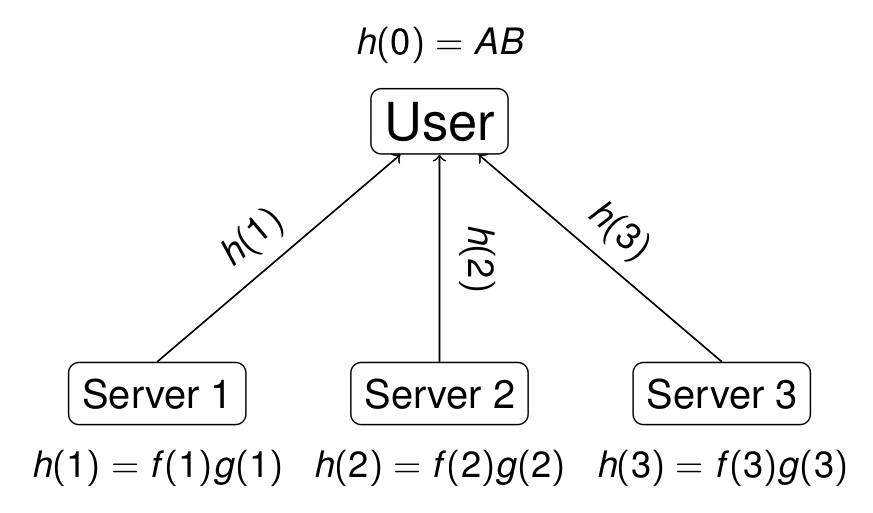
\includegraphics[width=0.8\textwidth]{poly_code.png}
            \end{figure}
            \item $f(x) = A + Rx$
            \item $g(x) = B + Sx$
            \item $h(x) = f(x) \cdot g(x) = AB + \left(AS + RB\right) + RSx^2$
        \end{itemize}
        
    \end{frame}

    \begin{frame}
        
        \frametitle{Разбиение матриц}
        Рассмотрим разбиение матриц:
        \begin{itemize}
            \item<1-> Первого множителя -- по строкам
            \begin{equation*}
                A = 
                \begin{bmatrix}
                    A_1 \\ \vdots \\ A_K
                \end{bmatrix}
            \end{equation*}
            \item<2-> А второго -- по столбцам
            \begin{equation*}
                B = 
                \begin{bmatrix}
                    B_1 & \dots & B_L
                \end{bmatrix}
            \end{equation*}
            \item<3-> Их произведение будет иметь вид
            \begin{equation*}
                AB =
                \begin{bmatrix}
                    A_1B_1 & \dots & A_1B_L \\
                    \vdots & \ddots & \vdots \\
                    A_K B_1 & \dots & A_K B_L
                \end{bmatrix}
            \end{equation*}
            \end{itemize}
    \end{frame}

    \begin{frame}
        \frametitle{Не всякие многочлены подходят}
        \begin{itemize}
            \item<1-> $f(x) = A_1 + A_2x + A_3x^2 + R_1x^3 + R_2x^4$
            \item<2-> $g(x) = B_1 + B_2x + B_3x^2 + S_1x^3 + S_2x^4$
            \item<3-> $h(x) = A_1B_1 + \left(A_1B_2 + A_2B_1\right)x + \left(A_1B_3 + A_2B_2 + A_3B_1\right)x^3 + \cdots$
            \item<4-> Нельзя получить, например, $A_1B_2$
        \end{itemize}
    \end{frame}
    
\begin{frame}
    \frametitle{Степени используемых многочленов}
    Пусть
    \begin{itemize}
        \item $f(x) = A_1x^{\alpha_1} + A_2x^{\alpha_2} + A_3x^{\alpha_3}$
        \item $g(x) = B_1x^{\beta_1} + B_2x^{\beta_2} + B_3x^{\beta_3}$
    \end{itemize}
    Тогда степени $h(x)$ будут образовывать таблицу
    \begin{figure}[h!]
        \centering
        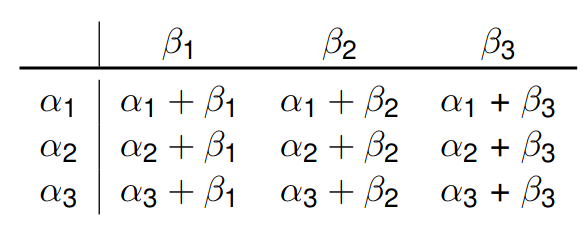
\includegraphics[width=0.7\textwidth]{deg_table.png}
    \end{figure}
\end{frame}

\begin{frame}
    \frametitle{Степени используемых многочленов}
    Общий случай таблицы степеней
    % \begin{equation*}
    %     \begin{matrix}
    %         & \beta_1 & \cdots & \beta_L & \beta_{L+1} & \cdots & \beta_{L+T} \\
    %         \alpha_1 & \alpha_1 + \beta_1 & \dots & \alpha_1 + \beta_L & \alpha_1 + \beta_{L+1} & \cdots & \alpha_1 + \beta_{L+T} \\
    %         \vdots & \vdots & \vdots & \vdots & \vdots & \vdots & \vdots
    %     \end{matrix}
    % \end{equation*}
    \begin{figure}[h!]
        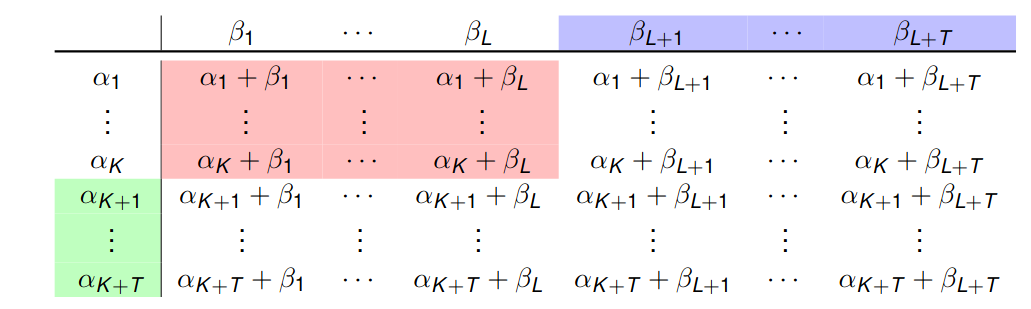
\includegraphics[width=0.9\textwidth]{deg_table_gen.png}
    \end{figure}
\end{frame}

\begin{frame}
    \frametitle{Степени используемых многочленов}
    \begin{itemize}
        \item Если $K \leqslant L$, построение таблицы степеней по следующей схеме:
        \begin{figure}[]
            \centering
            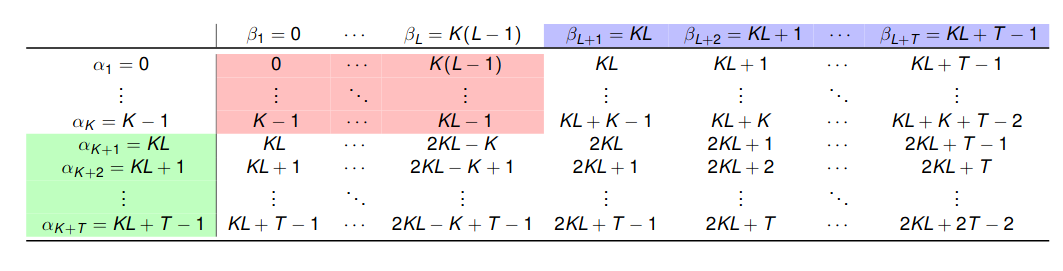
\includegraphics[width=0.9\textwidth]{gasp.png}
        \end{figure}
        \item Если $K > L$, меняем $\alpha$ и $\beta$ местами
    \end{itemize}
\end{frame}

\begin{frame}
    \frametitle{Полиномиальное кодирование: резюме}
    \begin{itemize}
        \item<1-> Имея матрицы $A$ и $B$, пользователь также задается параметрами $K$, $L$ и $T$ и вектором $\vec{a} = \left(a_1, \dots, a_N\right) \in \mathbb{F}^N_q$, где $N$ -- число серверов
        \item<2-> Пользователь разбивает $A$ по строкам на $K$ блоков $A_k$ и $B$~по столбцам на $L$ блоков $B_l$ и генерирует случайные матрицы $R_t$ и $S_t,\; t=\overline{1,T}$ подходящих размеров

        \item<3-> Пользователь строит 
        \begin{itemize}
            \item таблицу степеней $D$ по правилу, описанному выше
            % \item обобщенную матрицу Вандермонда $GV(\vec{a}, \mathcal{J})$
        \end{itemize}
        \item<4-> Воспользовавшись $D$, пользователь определяет многочлены 
        \begin{gather*}
            f(x) = \sum_{k=1}^K A_k x^{\alpha_k} + \sum_{t=1}^{T}R_t x^{\alpha_{K+t}} \\
            h(x) = \sum_{l=1}^L B_l x^{\beta_l} + \sum_{t=1}^{T}S_t x^{\beta_{L+t}}
        \end{gather*} 
    \end{itemize}
\end{frame}

\begin{frame}
    \frametitle{Полиномиальное кодирование: резюме}

    \begin{itemize}
        \item<1-> $h(x) = f(x)g(x)$ 
        \item<2-> Пользователь отправляет $f(a_n), g(a_n)$ на $n$-ый сервер, где вычисляется произведение $f(a_n)g(a_n) = h(a_n)$
        \item<3-> Интерполируя, пользователь восстанавливает многочлен $h(x)$ и получает $A_k B_l$ из его коэффициентов
        \item<4-> Таким образом, пользователь имеет произведение $AB$

    \end{itemize}

\end{frame}

\end{document}